\chapter{Particle Reconstruction and Identification}
\label{ch:part_reco}

With a design luminosity of $1.0 \times 10^{34}$ cm\textsuperscript{-2}s\textsuperscript{-1}, and a peak Run-2 instantaneous luminosity of $2.0 \times 10^{34}$ cm\textsuperscript{-2}s\textsuperscript{-1}, reconstructing and identifying the products of LHC $pp$ collisions is one of the most complex tasks for each LHC experiment. The accurate reconstruction and identification of physics objects lays the ground work for all subsequent physics analyses, so it is also one of the most fundamentally important tasks performed by an experiment. \par

Reconstruction is the process of combining raw and uncalibrated hits across various subsystems into specific unique objects. Two particular subsystems, the Inner Detector (ID) tracker and the calorimeter play particularly important roles and will be discussed in detail. Analysis of the properties of the reconstructed objects identifies them as photon, electrons, muons, or jets. While photons, electrons, and muons are fundamental particles, jets represent a collimated shower of many hadronic particles, whose definition is more flexible. Jet reconstruction, clustering and substructure are all of particular important to jet identification, and to the later content of this thesis. Finally, reconstruction also identifies missing transverse energy \met in events, which is a crucial variable for BSM physics searches. Figure \ref{fig:detector_objects} shows how the various physics objects listed here interact with various systems in the ATLAS detector. 

\begin{figure}
        \centering
	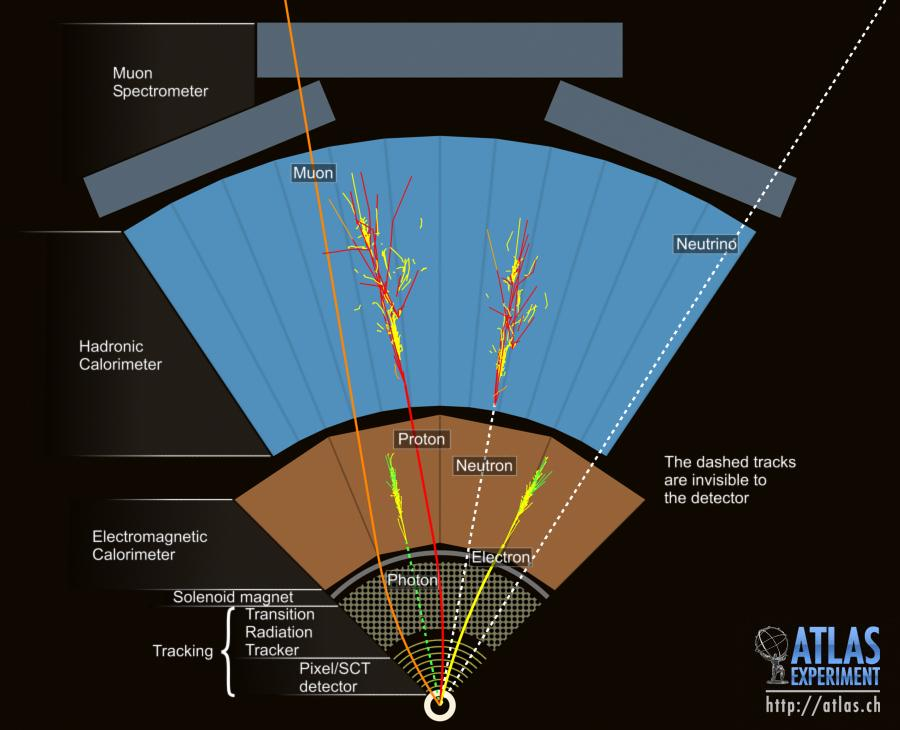
\includegraphics[width=0.7\textwidth]{figures/ch5/detector_objects}
	\caption{Graphic illustrating the various objects and high level features identified by ATLAS object reconstruction, and their interaction with different systems of the ATLAS detector \cite{detector_events}}
	\label{fig:detector_objects}
\end{figure}

\section{Inner Detector Tracks}
\label{sec:inner_det_tracks}
As the inner most layer of the detector, the ID measures charged particles close to the interaction point. The various hits of these charged particles throughout the ID are used to reconstruct \textit{tracks} which give the trajectories of charged particles. Track reconstruction begins by clustering hits in the Pixel and SCT detectors, and combining clusters from different radial laters of these detector. The multi-layer clusters form track \textit{seeds}, which provide initial estimates of measurements belonging to an individual track. The requirement of three points allows for a rough estimate of the track \pt to be made by calculating the curvature of the track and accounting of the magnetic field in the ID. \par

Tracks seeds are subject to a variety of quality requirements, such as having a minimum estimated \pt and passing interaction region compatability criterion. If these requirements are satisfied, the track seeds are passed to the track finding and fitting algorithms. The interplay of these three track reconstruction steps is illustrated in Figure \ref{fig:track_reco}. 

\begin{figure}
        \centering
	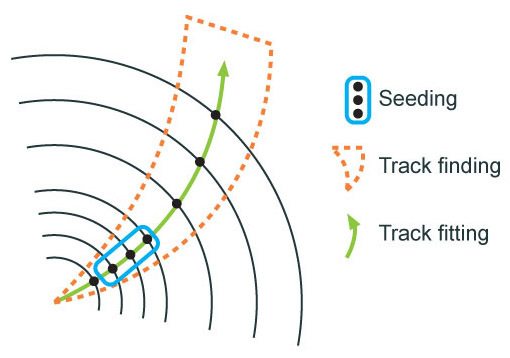
\includegraphics[width=0.6\textwidth]{figures/ch5/track_reco}
	\caption{Track reconstruction seeding, finding and fitting illustration \cite{track_finding}}
	\label{fig:track_reco}
\end{figure}

\section{Photons and Electrons}
Photons and electrons shower in the LAr calorimeter, and are identified by the energy deposits they leave there. Energy deposits in a collection of nearby cells are termed \textit{clusters}, which become the starting point for electron and photon reconstruction \cite{electron_photon}. The clustering algorithm begins when the energy deposit in a certain cell exceeds the noise threshold with a significance of 4$\sigma$. The algorithm then collects neighboring cells which have an energy deposit exceeding the noise threshold with a significance of 2$\sigma$, creating a topo-cluster. Next, these topo-clusters are matched to ID tracks, created as described in Section \ref{sec:inner_det_tracks}. The location of the topo-cluster defines a region of interest (ROI) in the ID, where additional modified track reconstruction algorithms are run in the case that no associated tracks are found. Any ID tracks associated to the topo-cluster are retrofit to allow for additional energy loss due to bremsstrahlung. A converted photon track reconstruction algorithm is run to check for tracks coming from secondary vertices consistent with converted photons. The secondary vertices are constructed from two opposite charged tracks consistent with a massless particle, or from one track without any hits in the innermost layer of the ID. \par

For electron identification, the EM cluster is required to match ID tracks that originate from the primary vertex at the interaction point. For photon identification, the EM cluster can either be matched to tracks coming from a secondary vertex (converted photon), or matched to no tracks (unconverted photon). Figure \ref{fig:electron_photon_id} illustrates these three cases for EM object identification. \par

\begin{figure}
        \centering
	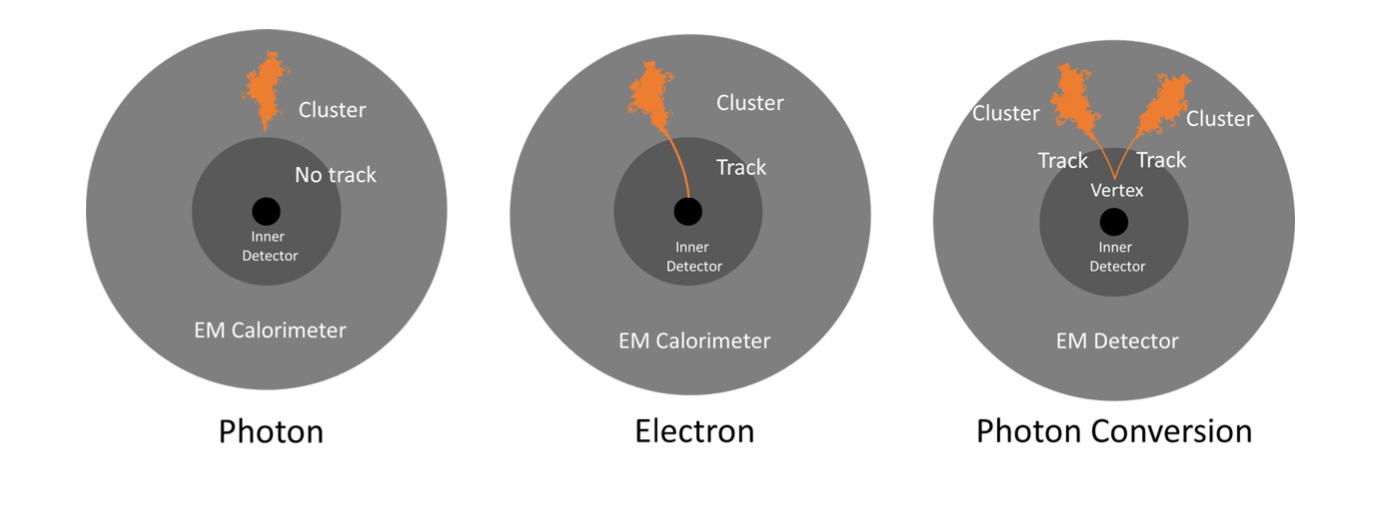
\includegraphics[width=0.8\textwidth]{figures/ch5/electron_photon_id}
	\caption{Four types of muon track candidates \cite{electron_photon_id}. }
	\label{fig:electron_photon_id}
\end{figure}

\textit{Superclusters} are built separately for photons and electrons, based on the combined topo-cluster and ID track information. First, the EM topo-clusters are tested to see if they meet the minimum requirements to become electron or photon seed clusters. For electrons, the cluster must have a minimum \et~of 1 GeV, and must be matched to a track with at least 4 hits in the silicon tracking detectors. For photons, the cluster must have an \et~greater than 1.5 GeV. If the seed cluster requirements are met, the algorithm searches for satellite clusters, which can arise from bremsstrahlung radiation. If the satellite clusters pass the positional, energy and tracking requirements to be associated with the proto-cluster, they are combined into a supercluster. \par

Electron and photon objects are identified from the superclusters after energy calibration and position corrections are applied. Because photon and electron superclusters are built independently, some clusters can produce both a photon and an electron. In this case an ambiguity resolution procedure is applied to determine if the supercluster can be easily identified as only a photon (no tracks present) or only an electron (good tracks pointing to the primary vertex). In some cases, the identity of the cluster is still ambiguous, in which case both a photon and electron object are created for analysis and flagged as ambiguous. Energy, shower shape, and other analysis variables are calculated from the supercluster and saved with the electron or photon object. 

\section{Muons}
Muons are identified through the tracks and energy deposits they leave in the ID, calorimeters, and Muon Spectrometer (MS). Muon identification begins in the Muon Drift Tube chambers by performing a straight line fit between the hits found in each layer, creating \textit{segments}. Segments in the middle layers are then used a seeds for the track building algorithm, which searches for compatible combinations of segments based on their relative positions and angles. A $\chi^2$ fit is performed on each track candidate \cite{muon_reco}. Based on the $\chi^2$ criteria, hits are removed or added such that the track contains as many hits as possible while satisfying the fit criteria. \par

The MS track candidates are combined with track information from the ID and calorimeters according to various algorithms based on the information available from each subdetector. Four different types of muons arise from the various reconstruction algorithms: 
\begin{itemize}
  \item Combined muon: a muon track identified through independent track reconstruction in the ID and MS, where the combined track is formed using a global refit that uses hit information from both detectors. Most muons are constructed through an outside-in procedure, in which a muon track candidate is identified in the MS and then an associated track is found in the ID. A complementary inside-out procedure is also implemented and identifies additional muons.
  \item Segment-tagged muon: an ID track is identified as a muon if when extrapolated out to the MS (following the inside-out global fit procedure) it is matched to at least one local MS segment. 
  \item Calorimeter-tagged muon: an ID track is identified as a muon if it is matched to a calorimeter energy deposit that is compatible with a minimum-ionizing particle. This muon identification has the lowest purity, but it used in regions where the MS has only partial coverage due to cabling and service access routes.
  \item Extrapolated muons:  the muon is reconstruction only from the MS track and a requirement on compatibility with the primary interaction point. The muon track is required to cross at least two layers of the MS, and three layers in the forward region. These muons are mainly used to extend muon acceptance into the region 2.5 < $|\eta|$ < 2.7 where ID track information is not available.
\end{itemize}

Figure \ref{fig:muon_tracks} illustrates the four types of muon reconstruction. Overlap between reconstructed muons using ID tracks is resolved by giving preference to combined muons, then segment tagged muons, and finally calorimeter tagged muons. Overlap with extrapolated muons is resolved by giving preference to the muon with a better fit quality and higher number of tracks. \par

All muon track candidates are required to pass a series of quality selections to be identified in the final muon collection. The primary qualities considered are the $\chi^2$ goodness of fit for the global track, the difference in \pt~measurement between the ID and MS tracks, and the ratio between the charge and momentum of the tracks. The quality requirements help reject hadrons, primarily from kaon and pion decays. Muons candidates consistent with cosmic rays are also rejected.

\begin{figure}[h]
        \centering
	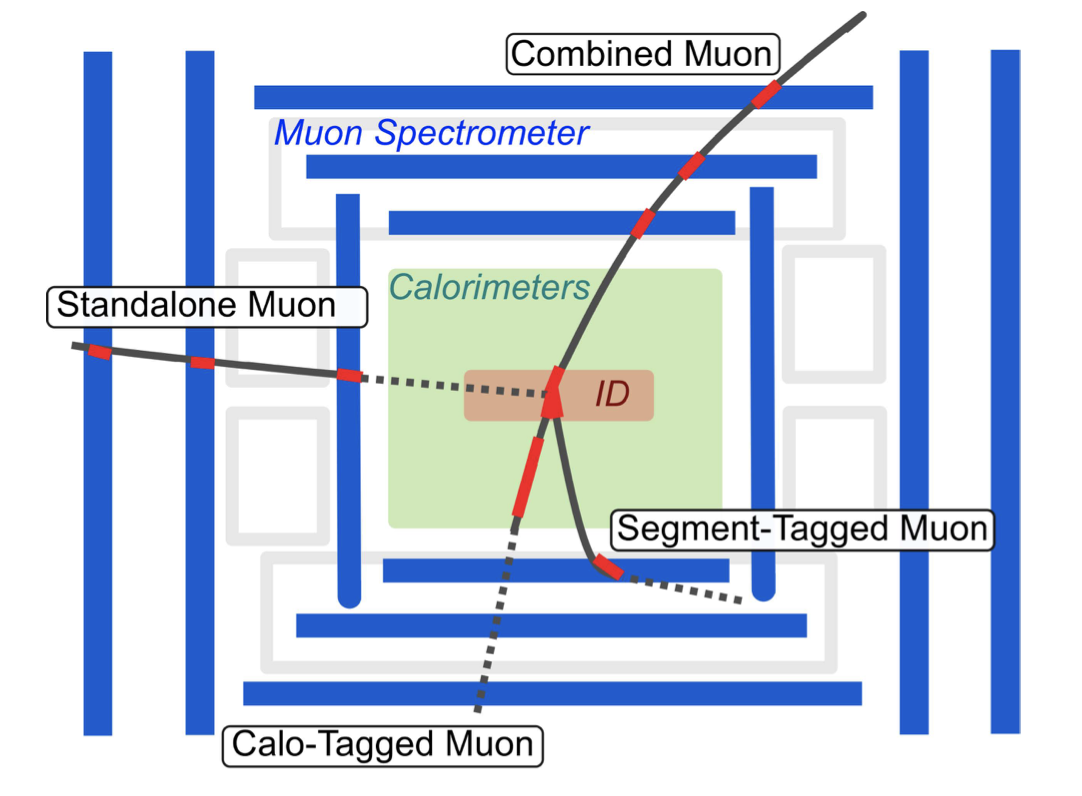
\includegraphics[width=0.6\textwidth]{figures/ch5/muon_tracks}
	\caption{Four types of muon track candidates \cite{muon_id}. }
	\label{fig:muon_tracks}
\end{figure}

\section{Jets}
The protons accelerated in the LHC are composed of quarks and gluons, and thus their collisions often result in the release of energetic quarks and gluons, collectively termed \textit{partons}. The energetic partons can radiate additional gluons, and these gluons can pair produce quarks in a process called \textit{fragmentation}. Fragmentation continues until the energy drops sufficiently that color conservation plays a dominant role. At that point, additional quarks and gluons are produced from vacuum to create neutral color states for the fragmented collection of partons. This process is known as \textit{hadronization} \cite{fragmentation}. The hadronized partons compose a collimated stream of particles, known as a \textit{jet}, which is then observed in the detector. The full process that produces jets is known as a \textit{parton shower}, and is illustrated in Figure~\ref{fig:parton_shower}. 

\begin{figure}[h]
        \centering
	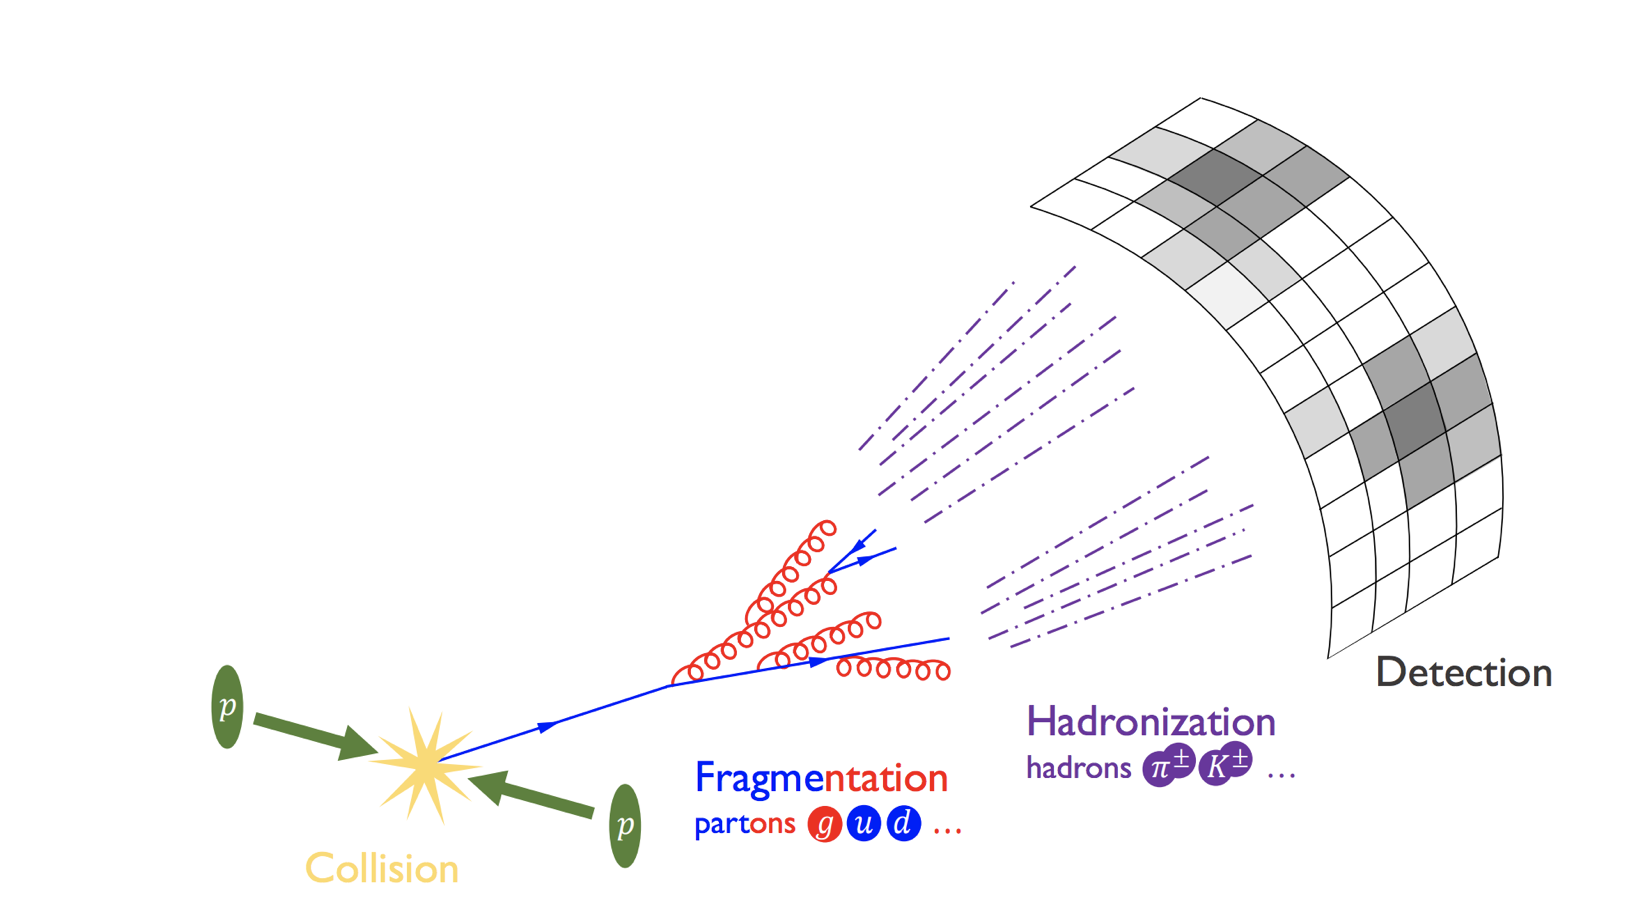
\includegraphics[width=0.6\textwidth]{figures/ch5/parton_shower}
	\caption{The fragmentation and hadronization processes undergone by a quark produced in a proton-proton collision \cite{frag_im}. }
	\label{fig:parton_shower}
\end{figure}

Jets are identified by the energy deposits they leave in the calorimeter, which are then matched to the tracks they leave in the ID. Jet reconstruction generally begins in the calorimeters, with the identification of \textit{topo-clusters}. Then jet reconstruction algorithms combine calorimeter information with tracking information. The anti-$k_t$ algorithm \cite{anti_kt} as provided by the FastJet library \cite{fast_jet} is generally used by the ATLAS experiment, with varying reconstruction radius settings. There are a variety of jet collections depending on the exact usage of calorimeter and tracking information in the reconstruction. Some common collections include particle flow iets(PFlow), track calo-cluster jets (TCC), EM topo-cluster jets (EMTopo), and unified flow object jets (UFO). Only particle flow jets will be discussed in greater detail due to their importance in this analysis. The following sections discuss jet identification in the calorimeters, particle flow jet construction using the anti-$k_t$ algorithm, jet clustering and jet substructure characteristics.

\subsection{Calorimeter Clusters}
\subsection{Particle Flow Reconstruction}
\subsection{Jet Clustering}
\subsection{Jet Substructure}

\section{Missing Transverse Energy}
